\subsection{自動判定の結果}
\label{sec:peculiar_eej_automatic_detection_results}
図\ref{fig:auto_visual_comparison}が目視確認と自動判定の検出結果である。
本手法による自動判定によって、これまで目視で確認されていた特異型EEJのイベントを定量的に抽出することが可能になった。
また、目視確認では見落とされていたイベントを追加で検出し、より正確な統計解析が可能となった。

下記が未発達型と突発型として抽出したイベント例である。




\begin{figure}[htbp]
  \centering
  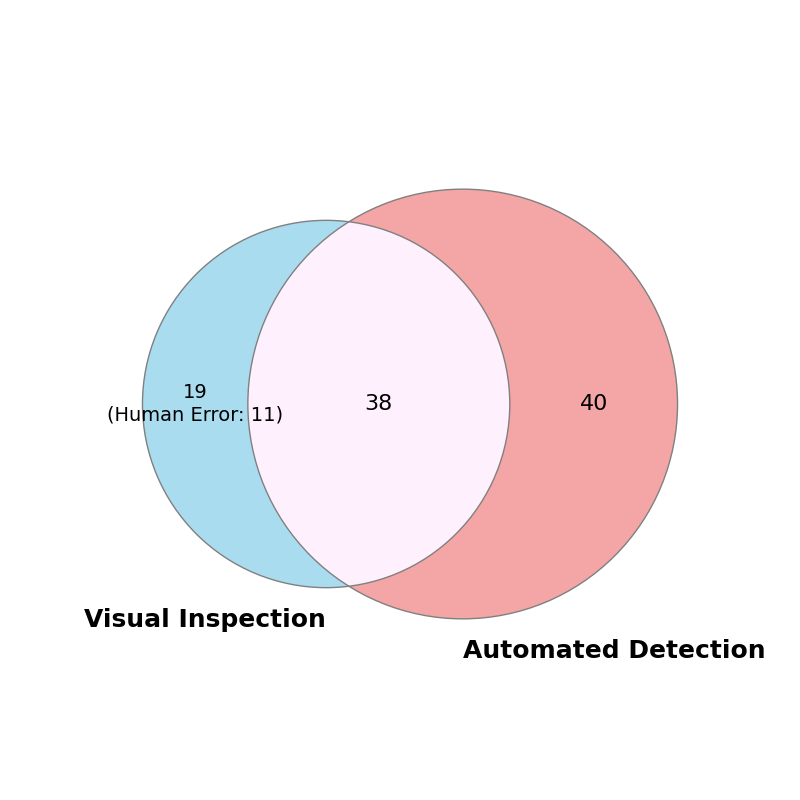
\includegraphics[width=0.8\textwidth]{figures/auto_visual.png}
  \caption{目視確認と自動判定の検出イベントの比較}
  \label{fig:auto_visual_comparison}
\end{figure}

また、観測地域、期間等の条件を変えた場合にも同様にして自動判定を行うことが可能になり、
特異型EEJのイベントを正確かつ効率的に抽出することが可能となった。
第\ref{sec:results}章では、これらのイベントの発生特性について、季節依存性、潮汐効果との関連について議論する。
